% Approved near-cubic scope, 12 September 2026. Compile twice with XeLaTeX.
% Previous annotated source/PDF are preserved in proposal_support/archive/.
% Evidence is regenerated by proposal_support/verify_corrections.py.
\documentclass[12pt,a4paper]{article}
\usepackage[margin=1in]{geometry}
\usepackage{fontspec}
\setmainfont{Times New Roman}
\usepackage{amsmath,amssymb,setspace,enumitem,titlesec}
\usepackage{tikz}
\usetikzlibrary{arrows.meta,positioning}
\usepackage[hidelinks]{hyperref}
\doublespacing
\titleformat{\section}{\normalfont\normalsize\bfseries}{\thesection.}{0.5em}{}
\titlespacing*{\section}{0pt}{6pt}{3pt}
\titleformat{\subsection}{\normalfont\normalsize\bfseries}{\thesubsection.}{0.5em}{}
\titlespacing*{\subsection}{0pt}{6pt}{3pt}
\setlist[enumerate]{leftmargin=1.6em,itemsep=0pt,parsep=0pt,topsep=2pt}
\setlength{\parindent}{0pt}
\setlength{\parskip}{3pt}
\setlength{\emergencystretch}{2em}
\hypersetup{pdftitle={Lie-Symmetry-Guided Corrections and Neural Approximation for Near-Cubic Saint-Venant-Exner Flows},pdfauthor={Carl}}
\input{proposal_support/evidence/pilot_values.tex}
\newcommand{\R}{\mathbb R}
\newcommand{\diag}{\operatorname{diag}}
\begin{document}

\begin{center}
\textbf{Lie-Symmetry-Guided Corrections and Neural Approximation\\
for Near-Cubic Saint--Venant--Exner Flows}\\
Carl \quad WKU MATH 4890\\
Proposed supervisor: Dr. Puneet Rana
\end{center}

\section{Research Problem}
Lie symmetry can select a special PDE solution family described by fewer independent variables. The question here is what remains useful when a model parameter changes and the selected symmetry no longer applies exactly. This project asks: \textbf{can a known cubic fluid reduction be continued through a regular, finite system of correction equations, and can a neural approximation represent those corrections reliably?}

Use the dimensionless Saint--Venant--Exner (SVE) system
\begin{equation}
\begin{aligned}
h_t+(hu)_x&=0,\\
u_t+uu_x+g(h+B)_x&=0,\\
B_t+\kappa\,\partial_x(u^{3+\delta})&=0.
\end{aligned}\label{eq:pde}
\end{equation}
Here $h>0$ is depth, $u>0$ velocity, $B$ bed elevation, and $g,\kappa>0$ are fixed. Reference scales are fixed before varying the exponent; only $\delta$ is perturbed. The cubic symmetry and solution family are established starting points \cite{sve}.

\section{Objectives}
\begin{enumerate}
\item Derive the cubic invariant family and identify its restricted scaling condition.
\item Construct logarithmic first-order corrections and prove their regularity and uniform PDE-residual order on a compact region.
\item Verify a numerical pilot, then compare analytical, classical numerical, and neural approximations of the correction profiles.
\end{enumerate}
The contribution being investigated is this model-specific construction and comparison, not a new universal PDE solver or a new maximal symmetry classification.

\newpage
\section{Methodology}
\subsection{Lie Reduction and Correction Profiles}
At $\delta=0$, the generator and its invariant solution form are
\begin{equation}
\begin{aligned}
X&=x\partial_x+u\partial_u+2h\partial_h+2B\partial_B,\\
u&=xv(t),\qquad h=x^2H(t),\qquad B=x^2C(t).
\end{aligned}\label{eq:invariants}
\end{equation}
The group scales $(x,u,h,B)$ by $(e^\rho,e^\rho,e^{2\rho},e^{2\rho})$, fixing $t$. Thus $u/x,h/x^2,B/x^2$ are invariants. The invariant-surface conditions $xu_x=u$, $xh_x=2h$, $xB_x=2B$ give \eqref{eq:invariants}, following classical Lie reduction \cite{olver}. Substitution yields
\begin{equation}
Y_0'=f(Y_0),\quad Y_0=(H,v,C)^T,\quad
f=\begin{pmatrix}-3Hv\\-v^2-2g(H+C)\\-3\kappa v^3\end{pmatrix}.
\label{eq:base}
\end{equation}
All coefficients are checked directly against \eqref{eq:pde}; specific discrepancies in the printed source formulas are recorded in the companion audit.

\textbf{Restricted scaling lemma.} For diagonal weights $(a,b,c,d,e)$ on $(t,x,u,h,B)$ at fixed $g,\kappa$, invariance requires $c=b-a$, $d=e=2c$, and $(m-3)c=0$. Nonzero amplitude scaling therefore requires $m=3$. For other exponents, simultaneous $t,x$ dilation still survives.

Since $u^{3+\delta}=u^3[1+\delta\log u+O(\delta^2)]$ and $\log(xv)=\log x+\log v$, set
\begin{equation}
W_\delta=D(x)\{Y_0(t)+\delta[p(t)+\log x\,q(t)]\},\quad
D(x)=\diag(x^2,x,x^2).
\label{eq:ansatz}
\end{equation}
Here $W=(h,u,B)^T$ and $p,q\in\R^3$. These are six correction functions of time. Set $p(t_0)=q(t_0)=0$ to retain the same initial fields for every exponent. This is perturbative continuation of an invariant family, not a verified approximate Lie generator \cite{disalvo}.

Arbitrary boundary data, shocks, full-PDE error theorems, and additional fluid models remain outside scope. The supporting derivation records the complete protocol and assumptions.

\newpage
\subsection{Correction Regularity and Main Proposition}
Splitting the coefficients of $\delta\log x$ and $\delta$ in \eqref{eq:pde} gives
\begin{equation}
q'=Jq+b,\qquad p'=Jp+Kq+c,\qquad J=Df(Y_0),
\label{eq:correction}
\end{equation}
where
\[
J=\begin{pmatrix}-3v&-3H&0\\-2g&-2v&-2g\\0&-9\kappa v^2&0\end{pmatrix},\quad
K=\begin{pmatrix}-v&-H&0\\-g&-v&-g\\0&-3\kappa v^2&0\end{pmatrix},
\]
\[
b=(0,0,-3\kappa v^3)^T,\qquad
c=(0,0,-\kappa v^3[1+3\log v])^T.
\]
The time-derivative matrix is $I_6$: no inversion of $J$ is needed. These are linear inhomogeneous ODEs, not a singular differential-algebraic system.

\textbf{Proposition.} Let $Y_0$ be a smooth solution of \eqref{eq:base} on $I=[t_0,T]$, with $H\ge H_{\min}>0$ and $v\ge v_{\min}>0$. Fix finite initial corrections and $K_x=[x_-,x_+]\subset(0,\infty)$. Then \eqref{eq:correction} has a unique solution on $I$. For sufficiently small $|\delta|$, \eqref{eq:ansatz} has positive depth and velocity and satisfies
\begin{equation}
\sup_{I\times K_x}\|F_\delta[W_\delta]\|_\infty\le C_*\delta^2,
\label{eq:bound}
\end{equation}
where $F_\delta$ is the original three-component residual and $C_*<\infty$ is independent of $\delta$ in a fixed small interval.

\textbf{Proof sketch.} Continuous coefficients give unique bounded linear-ODE corrections. Compactness and baseline positivity preserve positive fields for small $|\delta|$. Direct substitution cancels the zeroth and first parameter derivatives of $F_\delta[W_\delta]$. Its second parameter derivative is uniformly bounded on the resulting positive compact set; Taylor's remainder gives \eqref{eq:bound}.

The companion supplies the detailed proof. This is a classical correctness argument, not an intrinsic novelty claim. It bounds a residual, not distance to an exact noncubic PDE solution or global stability.

\newpage
\subsection{Numerical Verification}
For $g=1$, $\kappa=0.1$, use the independently checked control
\[
Y_0(t)=\left(\frac{1}{15t^2},\frac{2}{3t},\frac{2}{45t^2}\right)^T,
\quad 1\le t\le1.5,\quad 1\le x\le2.
\]
With zero initial corrections, DOP853 tolerance refinement changes profiles by $\PilotRefinement$; an independent matrix-exponential reference differs by $\PilotOracleDifference$. Time derivatives are obtained from the computed curve by refined finite differences, not by substitution of its ODE right-hand side.

The table shows maximum sampled original-PDE residuals on a $101\times61$ grid. Both signs with $|\delta|\in\{0.08,0.04,0.02,0.01,0.005\}$ pass the quadratic-order check. Positive values are shown; the uncorrected control instead has first-order defect.
\begin{center}
\input{proposal_support/evidence/pilot_table.tex}
\end{center}
These are sampled diagnostics, not validated supremum bounds or PDE solution errors. Depth and velocity remain positive at the tested points.

\begin{center}
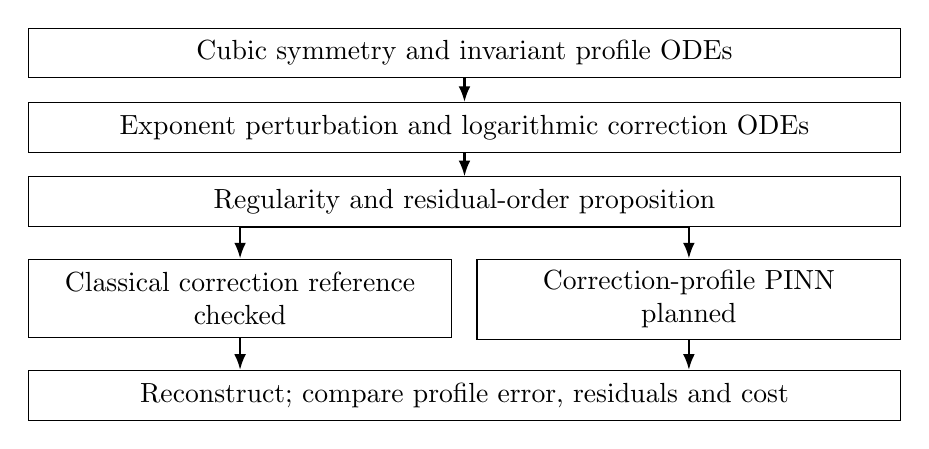
\begin{tikzpicture}[
  node distance=0.30cm,
  stage/.style={draw,align=center,text width=10.8cm,minimum height=0.63cm,inner sep=4pt},
  branch/.style={draw,align=center,text width=5.1cm,minimum height=1.0cm,inner sep=4pt},
  flow/.style={-{Latex[length=2mm]},thick}]
\node[stage] (base) {Cubic symmetry and invariant profile ODEs};
\node[stage,below=of base] (correction) {Exponent perturbation and logarithmic correction ODEs};
\node[stage,below=of correction] (proof) {Regularity and residual-order proposition};
\node[branch,below=0.40cm of proof.south west,anchor=north west] (classical) {Classical correction reference\\checked};
\node[branch,below=0.40cm of proof.south east,anchor=north east] (neural) {Correction-profile PINN\\planned};
\node[stage,below=0.40cm of classical.south west,anchor=north west] (check) {Reconstruct; compare profile error, residuals and cost};
\draw[flow] (base)--(correction);
\draw[flow] (correction)--(proof);
\draw[flow] (proof.south)-|(classical.north);
\draw[flow] (proof.south)-|(neural.north);
\draw[flow] (classical.south)--(classical.south |- check.north);
\draw[flow] (neural.south)--(neural.south |- check.north);
\end{tikzpicture}
\end{center}

\newpage
\subsection{Neural Approximation and Evaluation}
The network will learn $w=(q,p)$, not discover symmetries. For $s=t-t_0$, construct a time Taylor polynomial $P_N$ from \eqref{eq:correction} and use
\[
\widehat w_\theta=P_N(s)+s^{N+1}\mathcal N_\theta(s).
\]
Time-series order $N$ is distinct from first order in $\delta$. Taylor-plus-neural remainders are established \cite{taylor}; residual training follows PINNs \cite{pinn}. Symmetry-informed losses also have prior art \cite{liepinn}; this study instead hard-codes a baseline invariant shape and its derived corrections.

Compare $P_2$, classical integration, an initial-value-constrained PINN, and the Taylor-plus-PINN. Use matched small tanh networks, three seeds, 128 collocation points, and a distinct 1001-point evaluation grid. Train on the six scaled coefficient residuals, without solution labels. Report correction-profile error against the classical reference, reconstructed-field differences, PDE residuals, positivity, and training/evaluation cost.

Neural approximations do not automatically inherit \eqref{eq:bound}. For bounded smooth corrections on the same positive compact region, if
$r_q=\widehat q'-J\widehat q-b$ and $r_p=\widehat p'-J\widehat p-K\widehat q-c$, then
\[
F_\delta[\widehat W_\delta]
=\delta D(x)[r_p+\log x\,r_q]+O(\delta^2).
\]
Thus a fixed coefficient defect can mask quadratic scaling at small $\delta$. Neural improvement is an empirical question; no network has been trained for this submission pilot.

\textbf{Work plan.} Weeks 1--3: derivation and literature comparison; 4--6: analytical and numerical checks; 7--10: neural experiments; 11--12: evaluation and writing.

\section{Expected Outcomes}
Expected deliverables are a checked derivation, a local residual proposition, a reproducible benchmark, and an honest neural comparison. Originality of the spatial-log construction requires further comparison; neither the classical proof nor combining known techniques establishes it.

\newpage
\begin{thebibliography}{9}
\raggedright
\setlength{\itemsep}{3pt}
\setlength{\parskip}{0pt}
\bibitem{sve}
A. Paliathanasis. ``Lie Symmetry Analysis of the One-Dimensional Saint-Venant-Exner Model.'' \emph{Symmetry}, 14(8), 1679, 2022.
\href{https://doi.org/10.3390/sym14081679}{doi:10.3390/sym14081679}.

\bibitem{olver}
P. J. Olver. \emph{Applications of Lie Groups to Differential Equations}. Second edition, Springer, 1993.
\href{https://doi.org/10.1007/978-1-4612-4350-2}{doi:10.1007/978-1-4612-4350-2}.

\bibitem{disalvo}
R. Di Salvo, M. Gorgone, and F. Oliveri. ``A consistent approach to approximate Lie symmetries of differential equations.'' \emph{Nonlinear Dynamics}, 91(1), 371--386, 2018.
\href{https://doi.org/10.1007/s11071-017-3875-5}{doi:10.1007/s11071-017-3875-5}.

\bibitem{taylor}
C. K. Nagesh, S. Sankaranarayanan, R. Kaur, T. Sahai, and S. Jha. ``Taylor-Model Physics-Informed Neural Networks (PINNs) for Ordinary Differential Equations.'' \emph{PMLR}, 288, 621--642, 2025.
\href{https://proceedings.mlr.press/v288/nagesh25a.html}{proceedings.mlr.press/v288/nagesh25a.html}.

\bibitem{pinn}
M. Raissi, P. Perdikaris, and G. E. Karniadakis. ``Physics-informed neural networks: A deep learning framework for solving forward and inverse problems involving nonlinear partial differential equations.'' \emph{Journal of Computational Physics}, 378, 686--707, 2019.
\href{https://doi.org/10.1016/j.jcp.2018.10.045}{doi:10.1016/j.jcp.2018.10.045}.

\bibitem{liepinn}
T. Akhound-Sadegh, L. Perreault-Levasseur, J. Brandstetter, M. Welling, and S. Ravanbakhsh. ``Lie Point Symmetry and Physics-Informed Networks.'' \emph{NeurIPS}, 36, 42468--42481, 2023.
\href{https://arxiv.org/abs/2311.04293}{arXiv:2311.04293}.
\end{thebibliography}
\end{document}
